
Code has emerged as an important application area for \llms{}, with a proliferation of code-specific models 
\citep{chen2021evaluating,austin2021program, 
nijkamp2022codegen, li2023starcoder, roziere2023code, deepseek-coder,  ridnik2024code, starcoder2} and their applications across various tasks such as program repair ~\citep{opencodeinterpreter, olausson2023demystifying}, optimization~\citep{madaan2023learning}, test generation~\citep{steenhoek2023reinforcement}, documentation~\citep{luo2024repoagent}, SQL~\citep{sun2023sql}.
In contrast with these rapid advancements, evaluations have remained relatively stagnant, and current benchmarks like 
\humaneval{} and \mbpp{} paint a misleading picture.
%However, when it comes to evaluating LLM's coding capabilities, current benchmarks like \humaneval{}, \mbpp{}, \apps{}, and \contests{} have not kept pace and may paint a skewed or misleading picture.
%Particularly, they only focus on natural language to code tasks and suffer from overfitting and data contamination challenges with benchmark samples present in the training dataset for the latest \llms{}. 
Firstly, while coding is a multi-faceted skill, these benchmarks only focus on code generation, thus overlooking broader code-related capabilities. 
Moreover, these benchmarks suffer from contamination or overfitting, as benchmark samples are present in the training datasets.
%For instance, ~\citep{gemini15} mentioned XXX and ~\cite{lmsys-contamination-paper} said YYY.
%Beyond this, these benchmarks have reported issues of ambiguous problems and insufficient evaluations.
%ambiguous problem statements, insufficient tests, only natural language to code tasks, and 
\begin{figure}[!t]
    \centering
    % 
\includegraphics[width=0.6\columnwidth]{figures/overview/live_evaluation_over_time.png}
    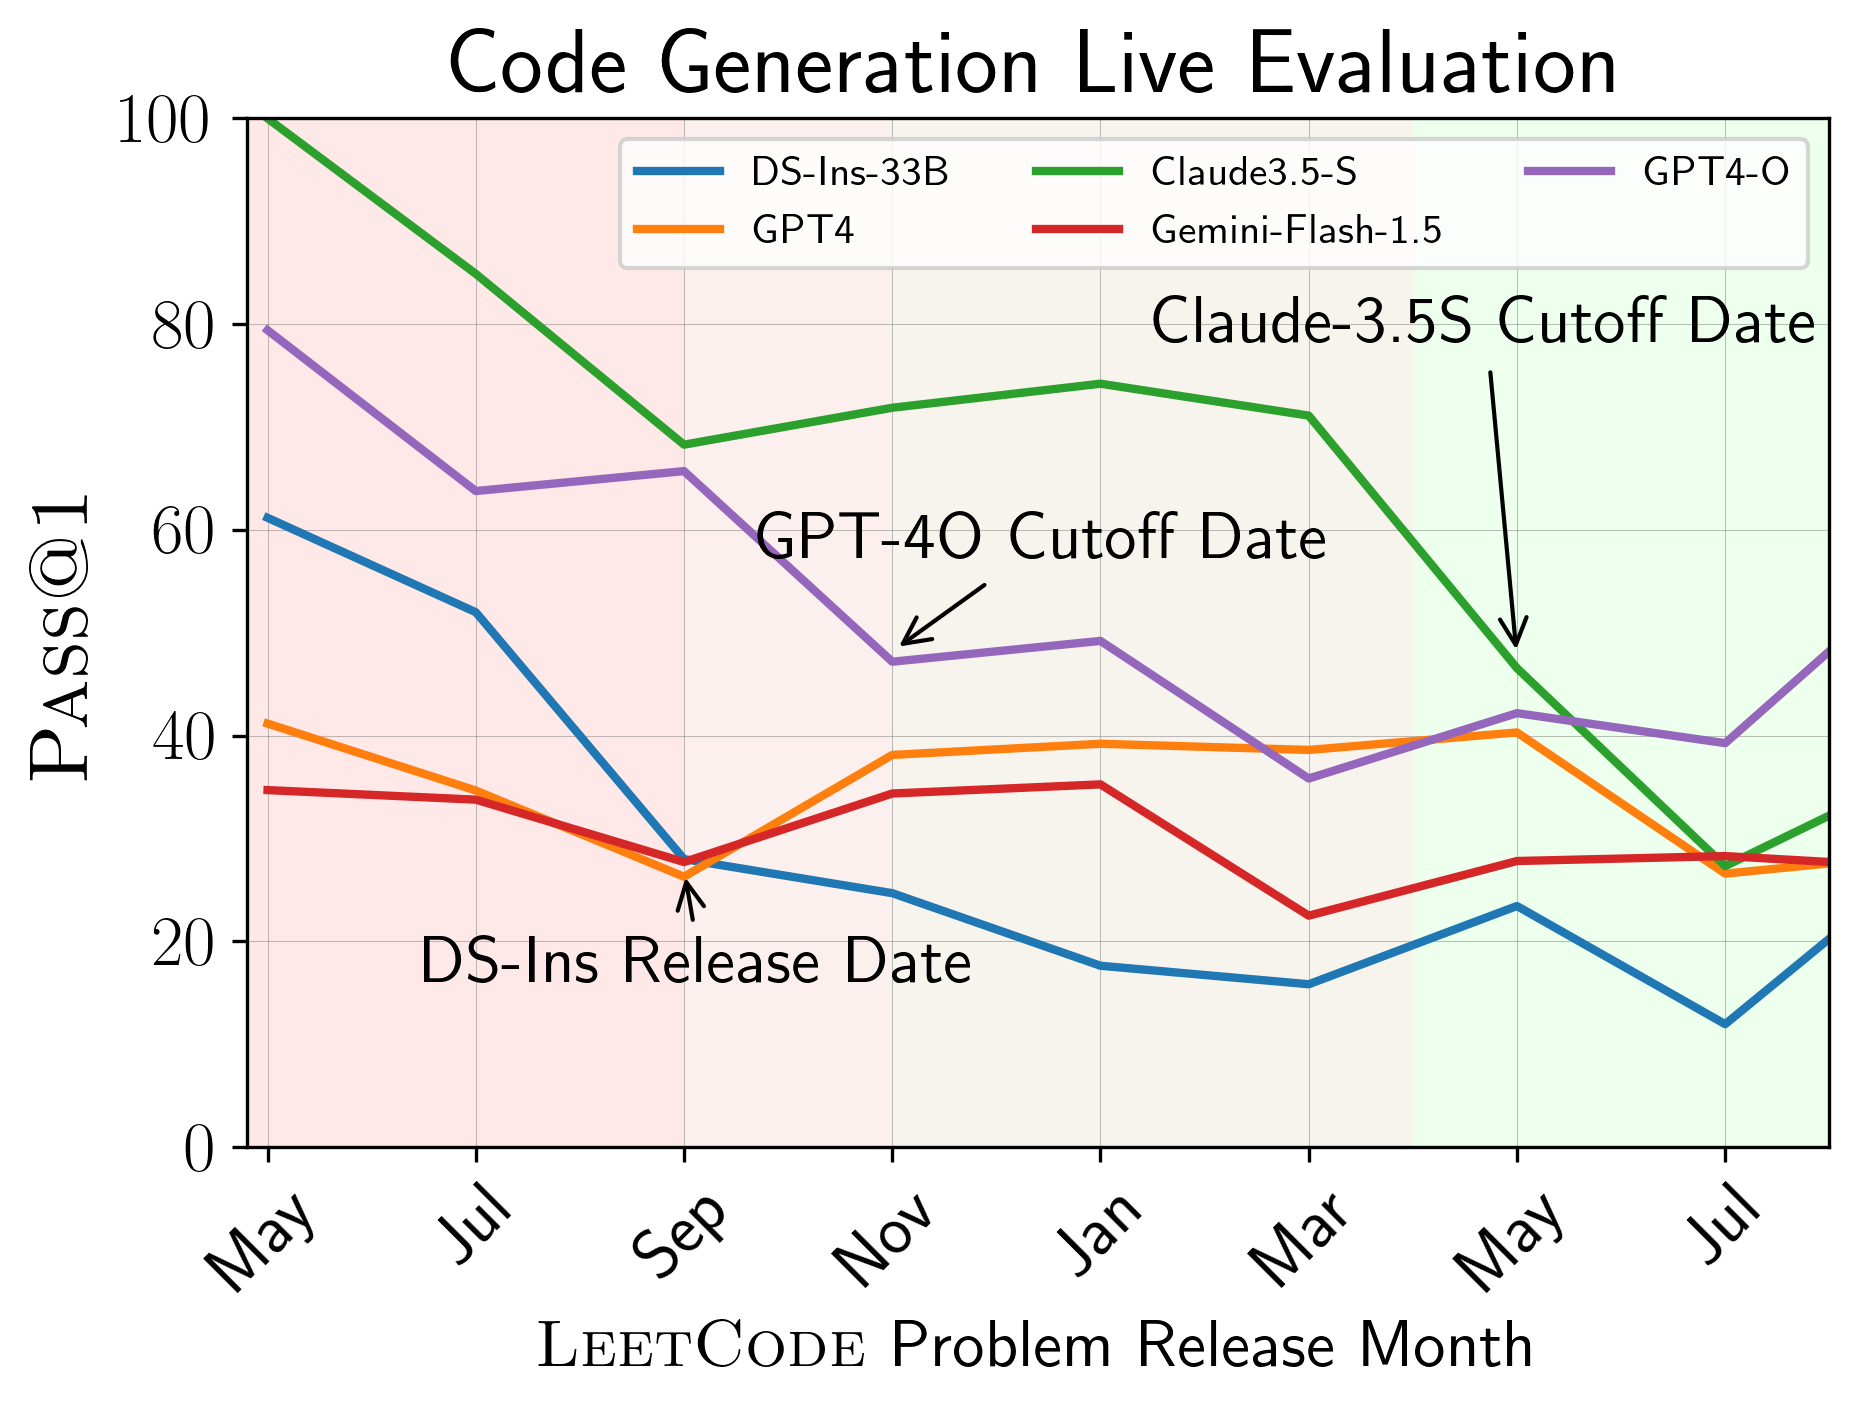
\includegraphics[width=0.50\linewidth]{figures/contamination_new/main_20_codegen_leetcode.png}
    \hfil%
        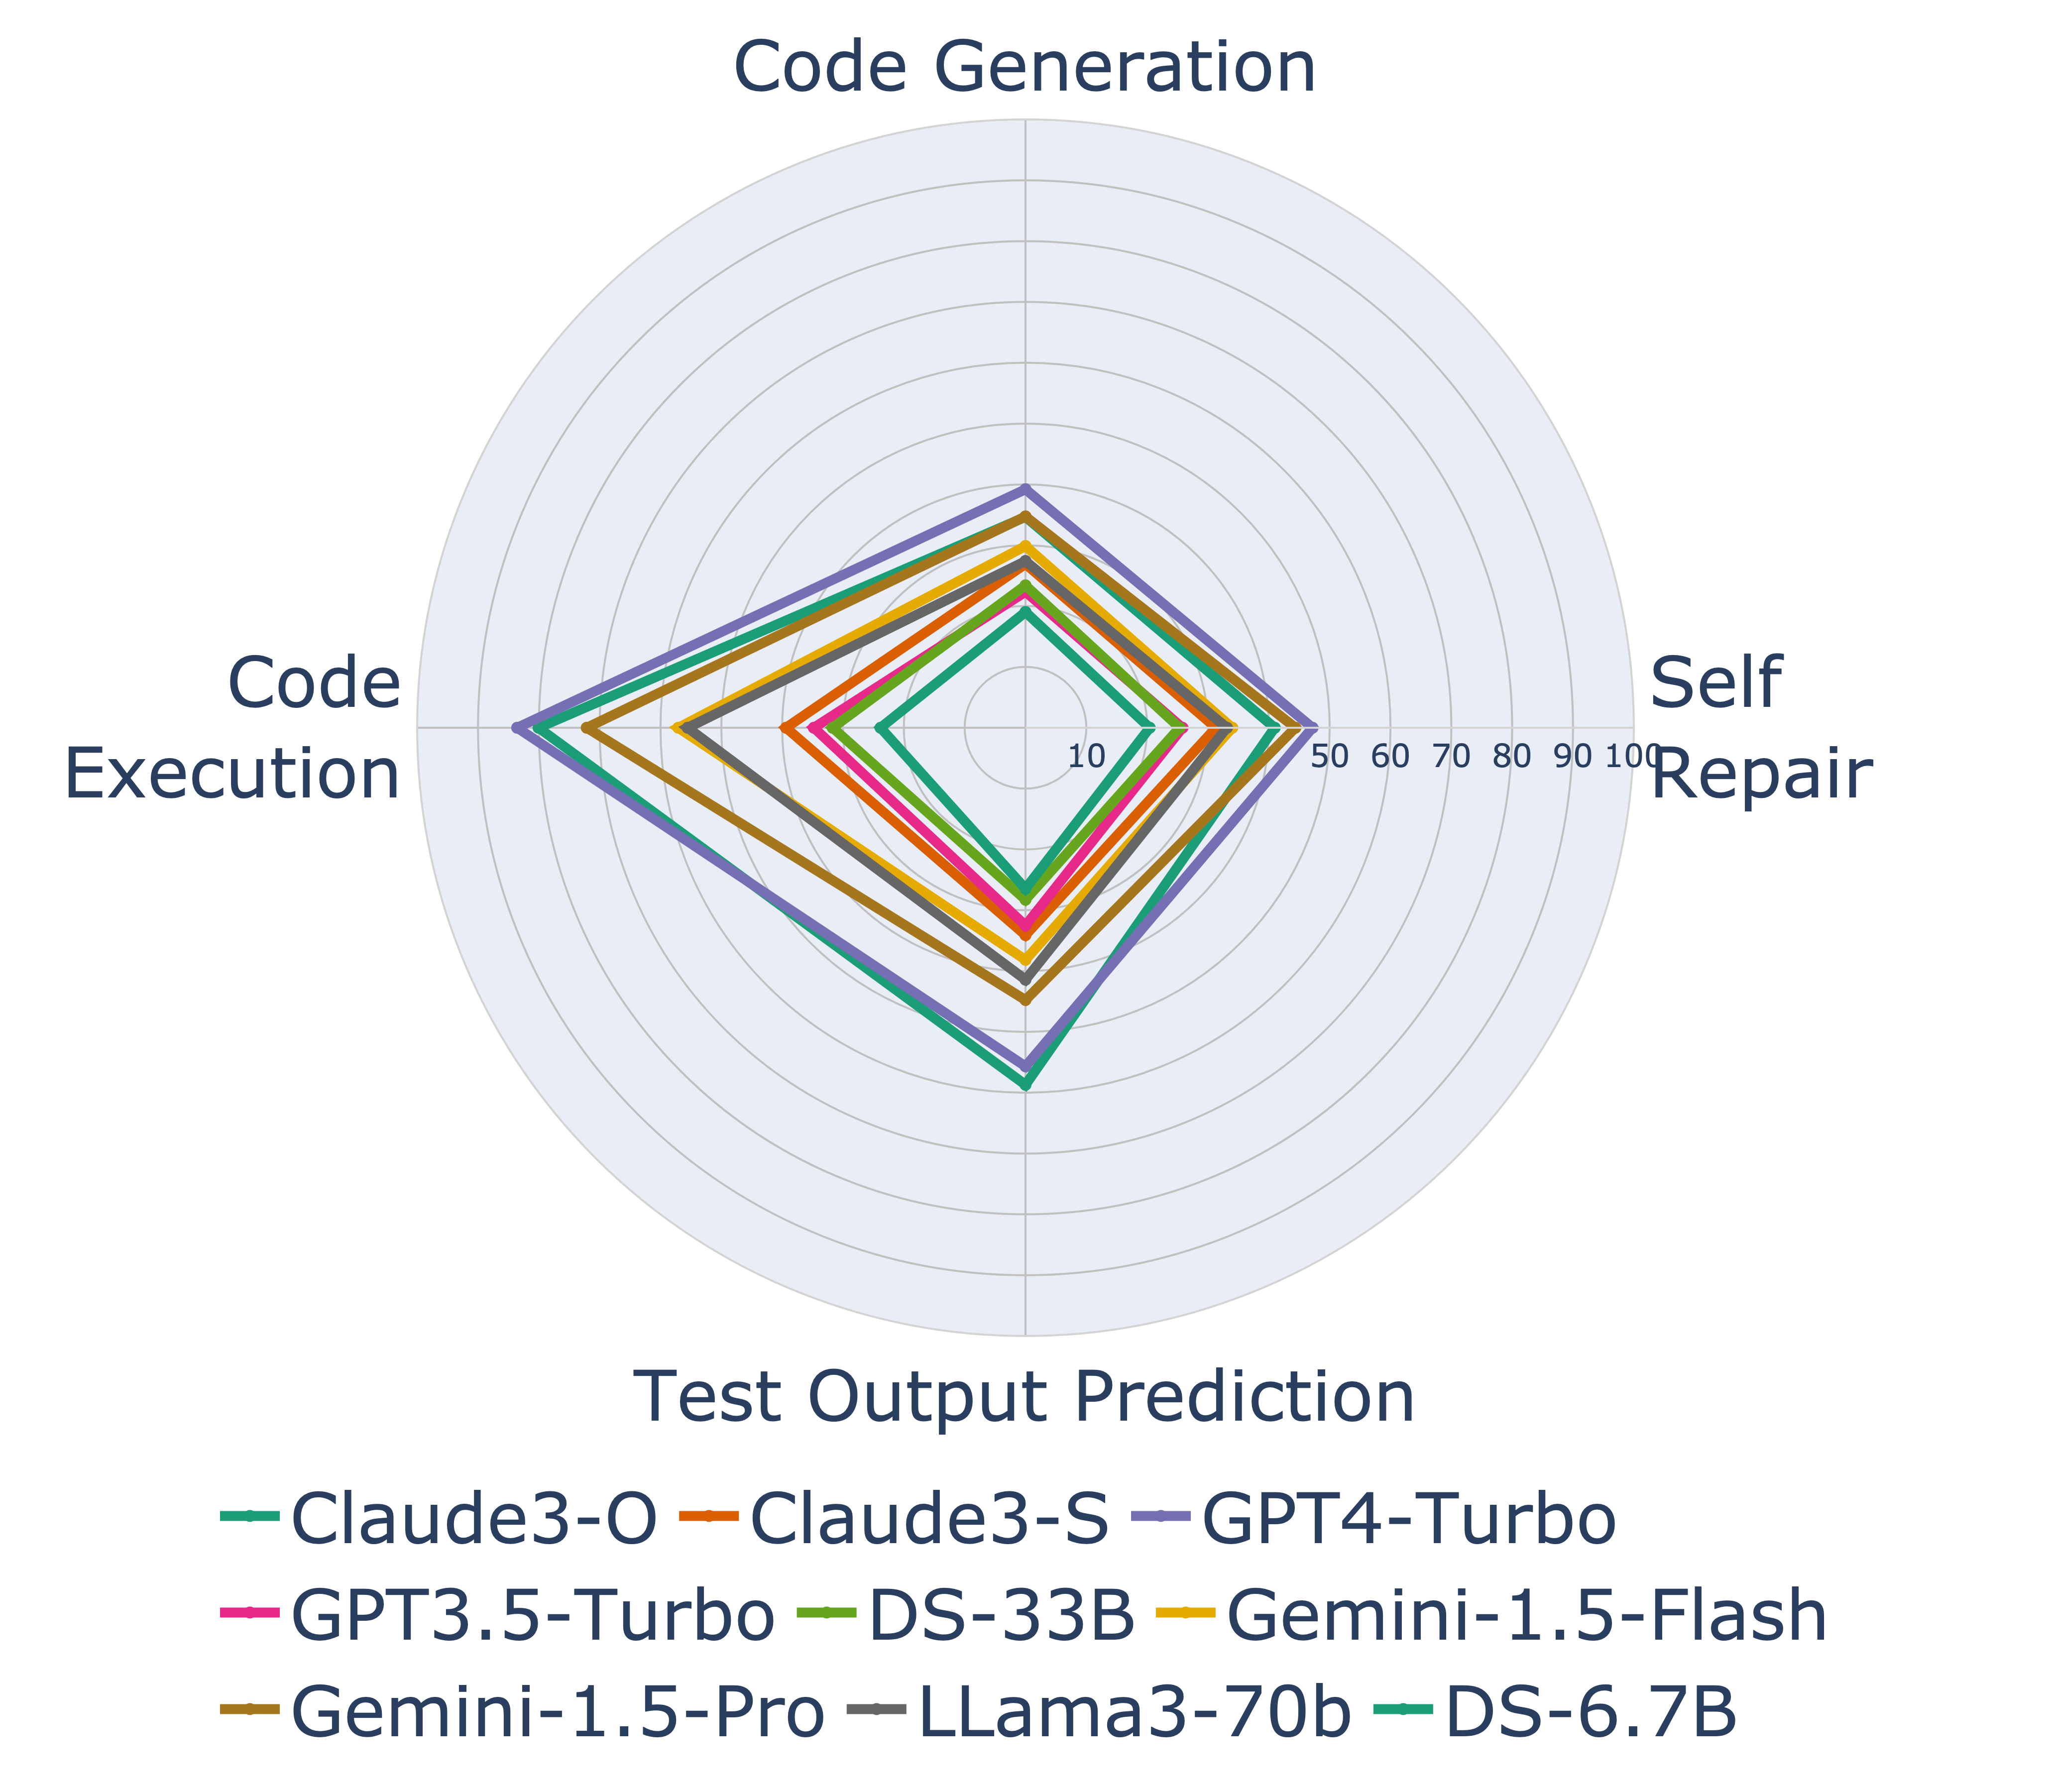
\includegraphics[width=0.435\linewidth]{figures/overview/tasks_radar.png}

        \vspace{-3pt}

    % 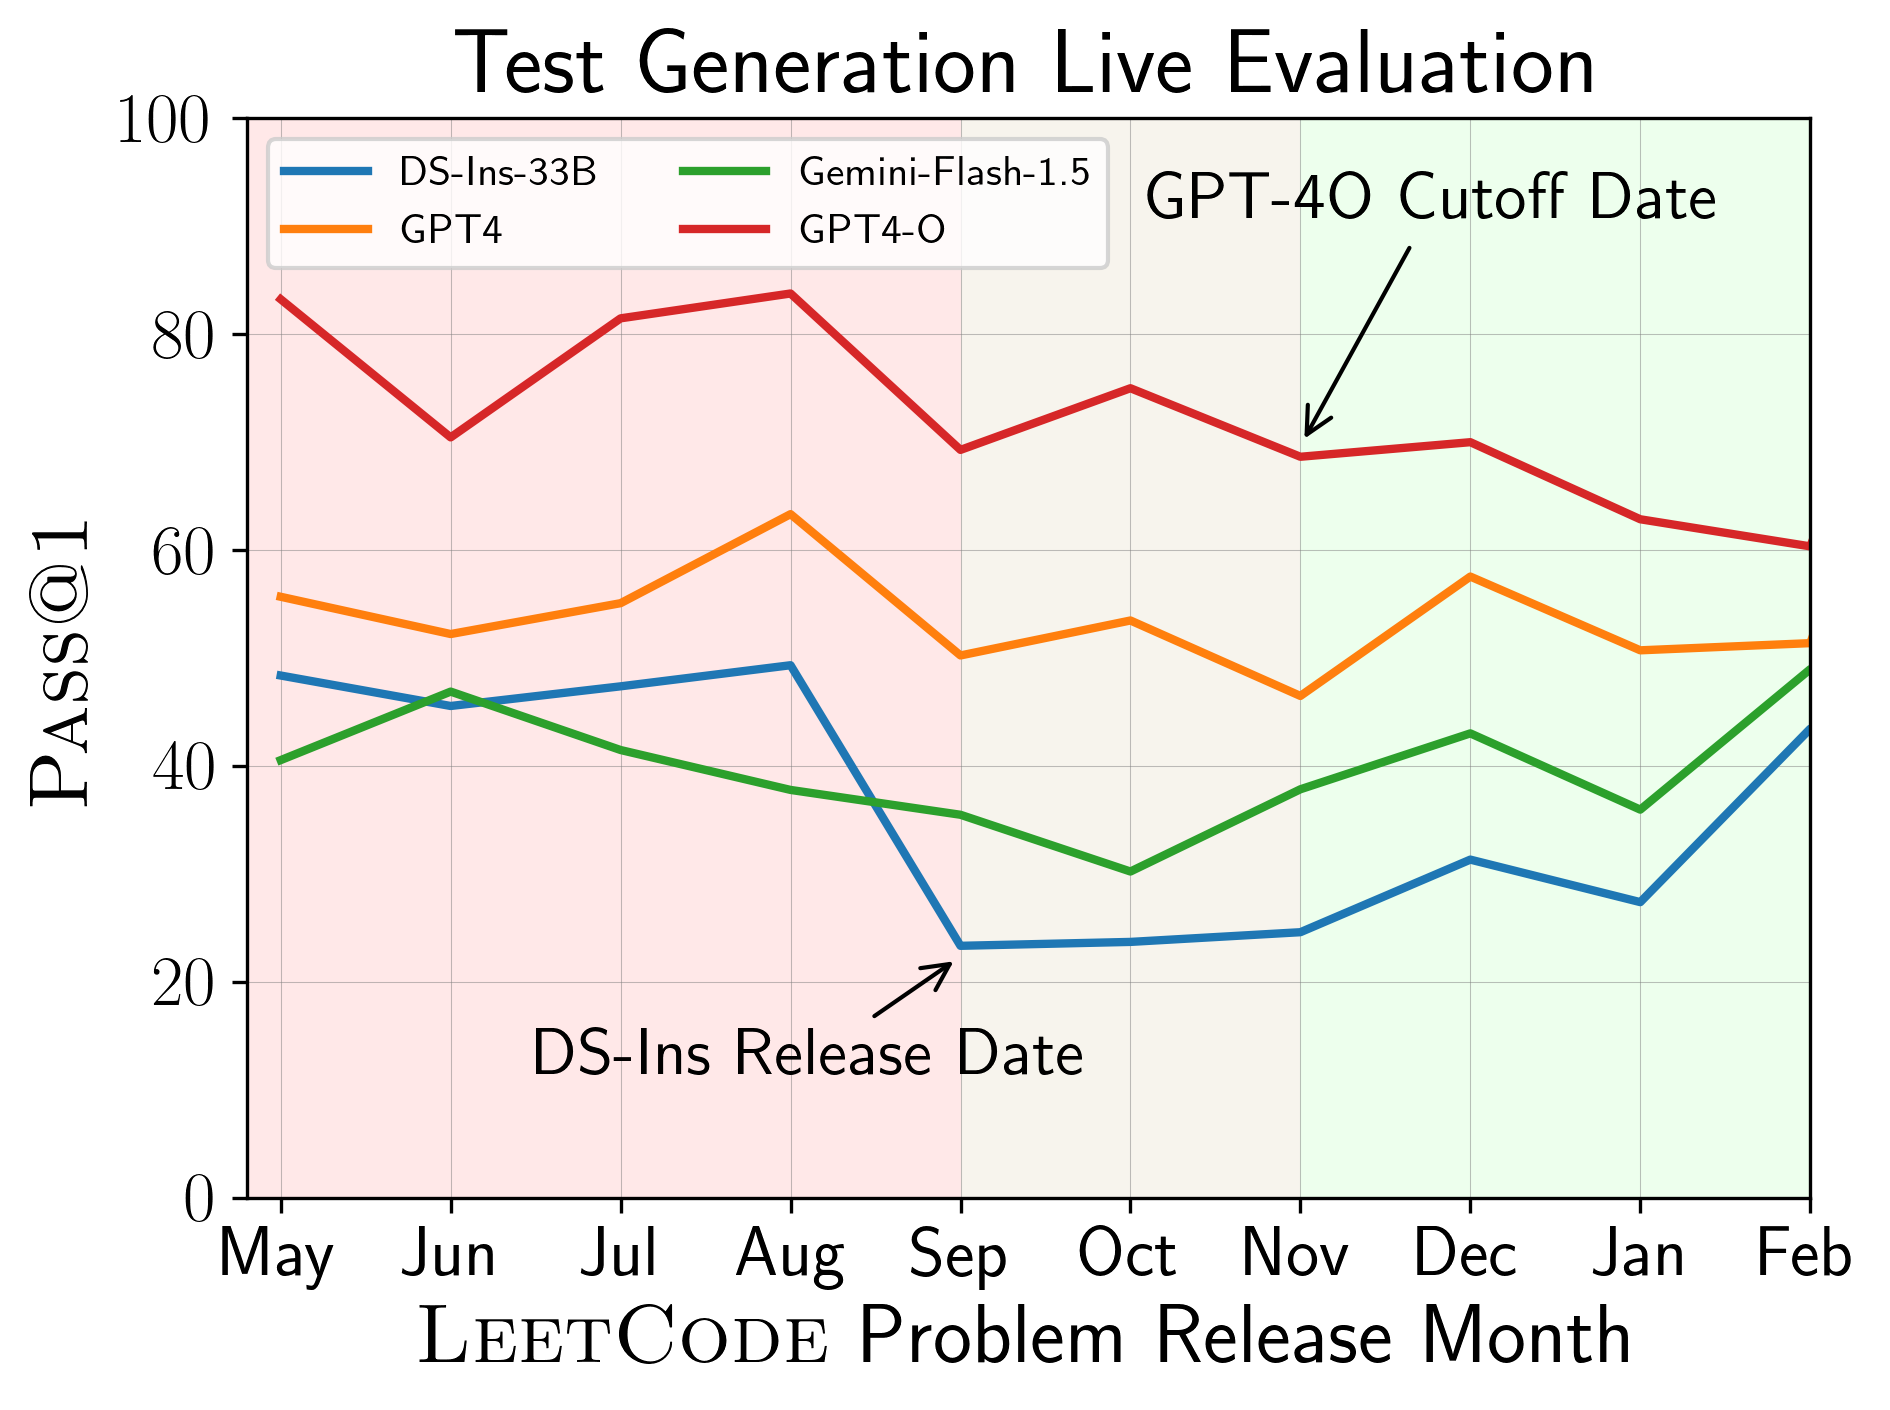
\includegraphics[width=0.49\linewidth]{figures/contamination_new/main_14_testgen_leetcode.png}%
    \caption{
        \textbf{Left.} \livecodebench{} comprises problems marked with release dates, allowing evaluations over different time windows.
        The figure depicts performances of \deepseek{}, \gptfouro{}, and \claudethrees{} models over bimonthly time windows ($\sim40$ \leetcode{} problems) showcasing a stark drop after their cutoff dates, highlighting contamination.
        Thus, we can detect and avoid contamination by evaluating models only on time-windows after the model's cutoff date (green region)\protect\footnotemark.
          \textbf{Right.} We evaluate \llms{} across 
        four scenarios that capture key coding capabilities necessary for building programming agents: code generation, repair, testing, and comprehension.
        %Specifically, we host four different scenarios, namely code generation, 
        %self-repair, code execution, and test output prediction.
        The figure depicts various model performances across the scenarios available in \livecodebench{} in a radial plot -- 
        highlighting relative differences changing across the scenarios.
        }
    \label{fig:contamination_main}
    \vspace{-10pt}
\end{figure}

\footnotetext{Note that for model comparisons -- performances are averaged across multiple months and platforms achieving a larger sample size.}
% \begin{figure}[!b]
    \centering
    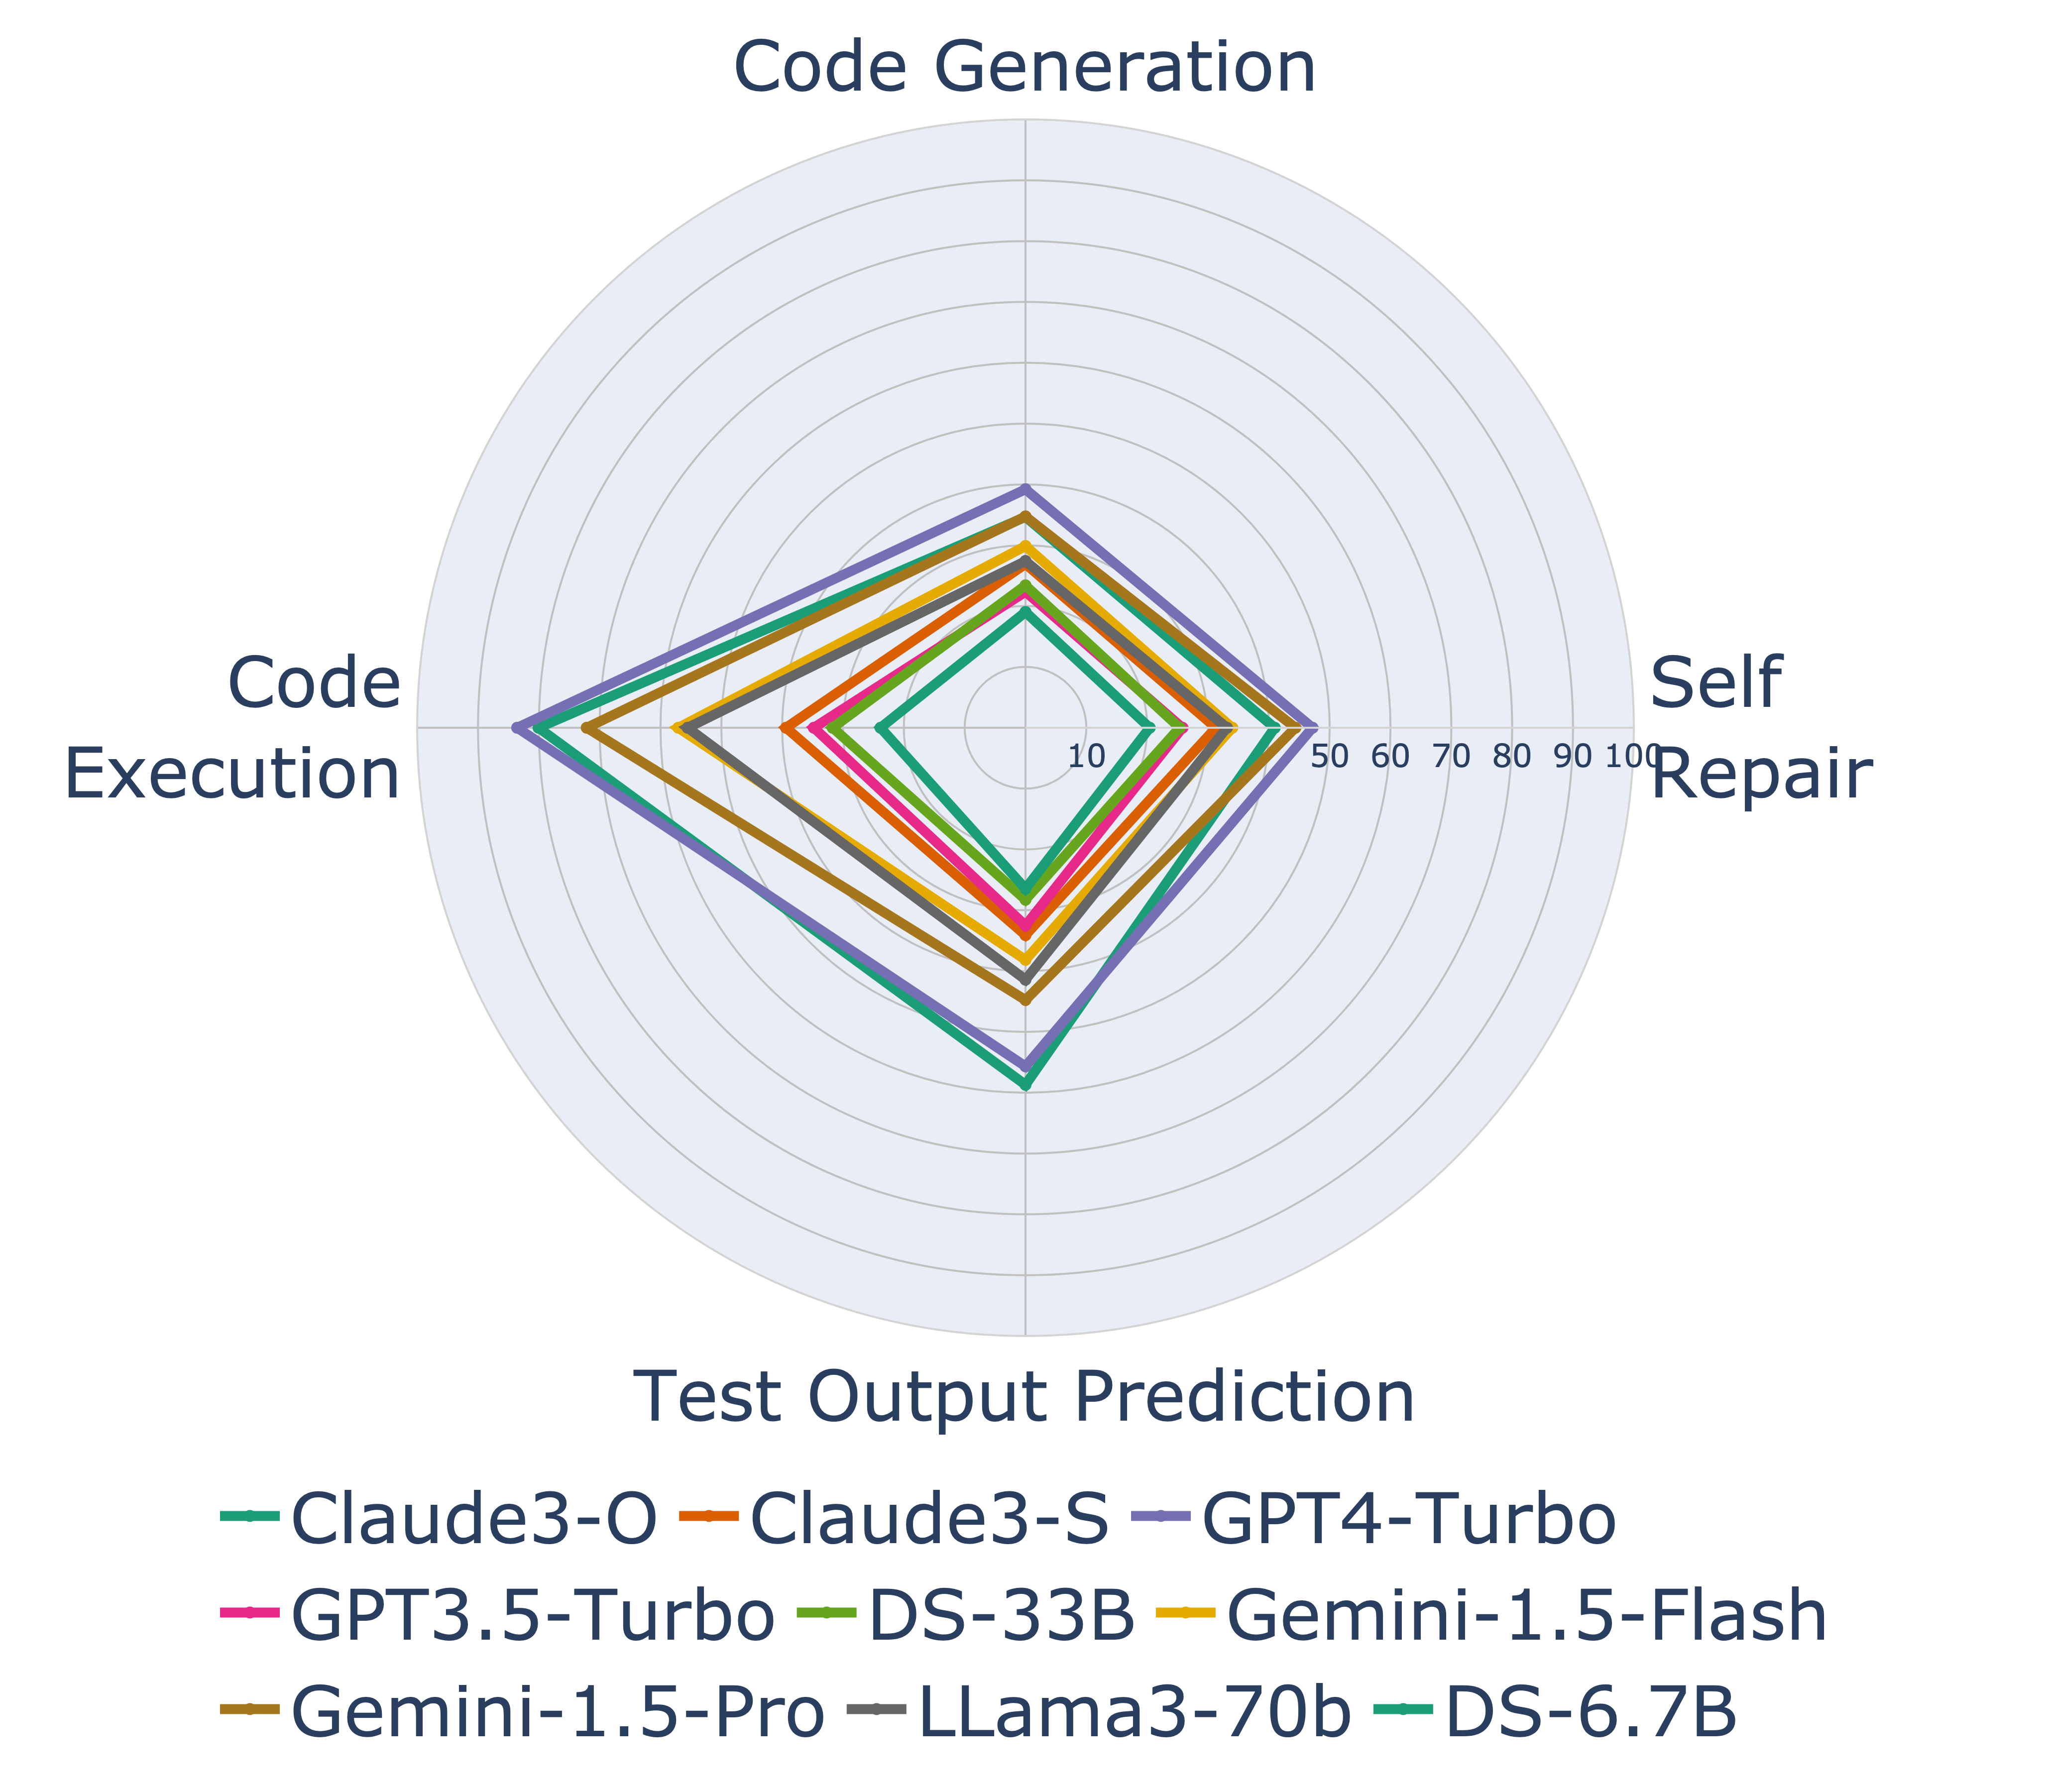
\includegraphics[width=0.47\linewidth]{figures/overview/tasks_radar.png}
    \hfil%
    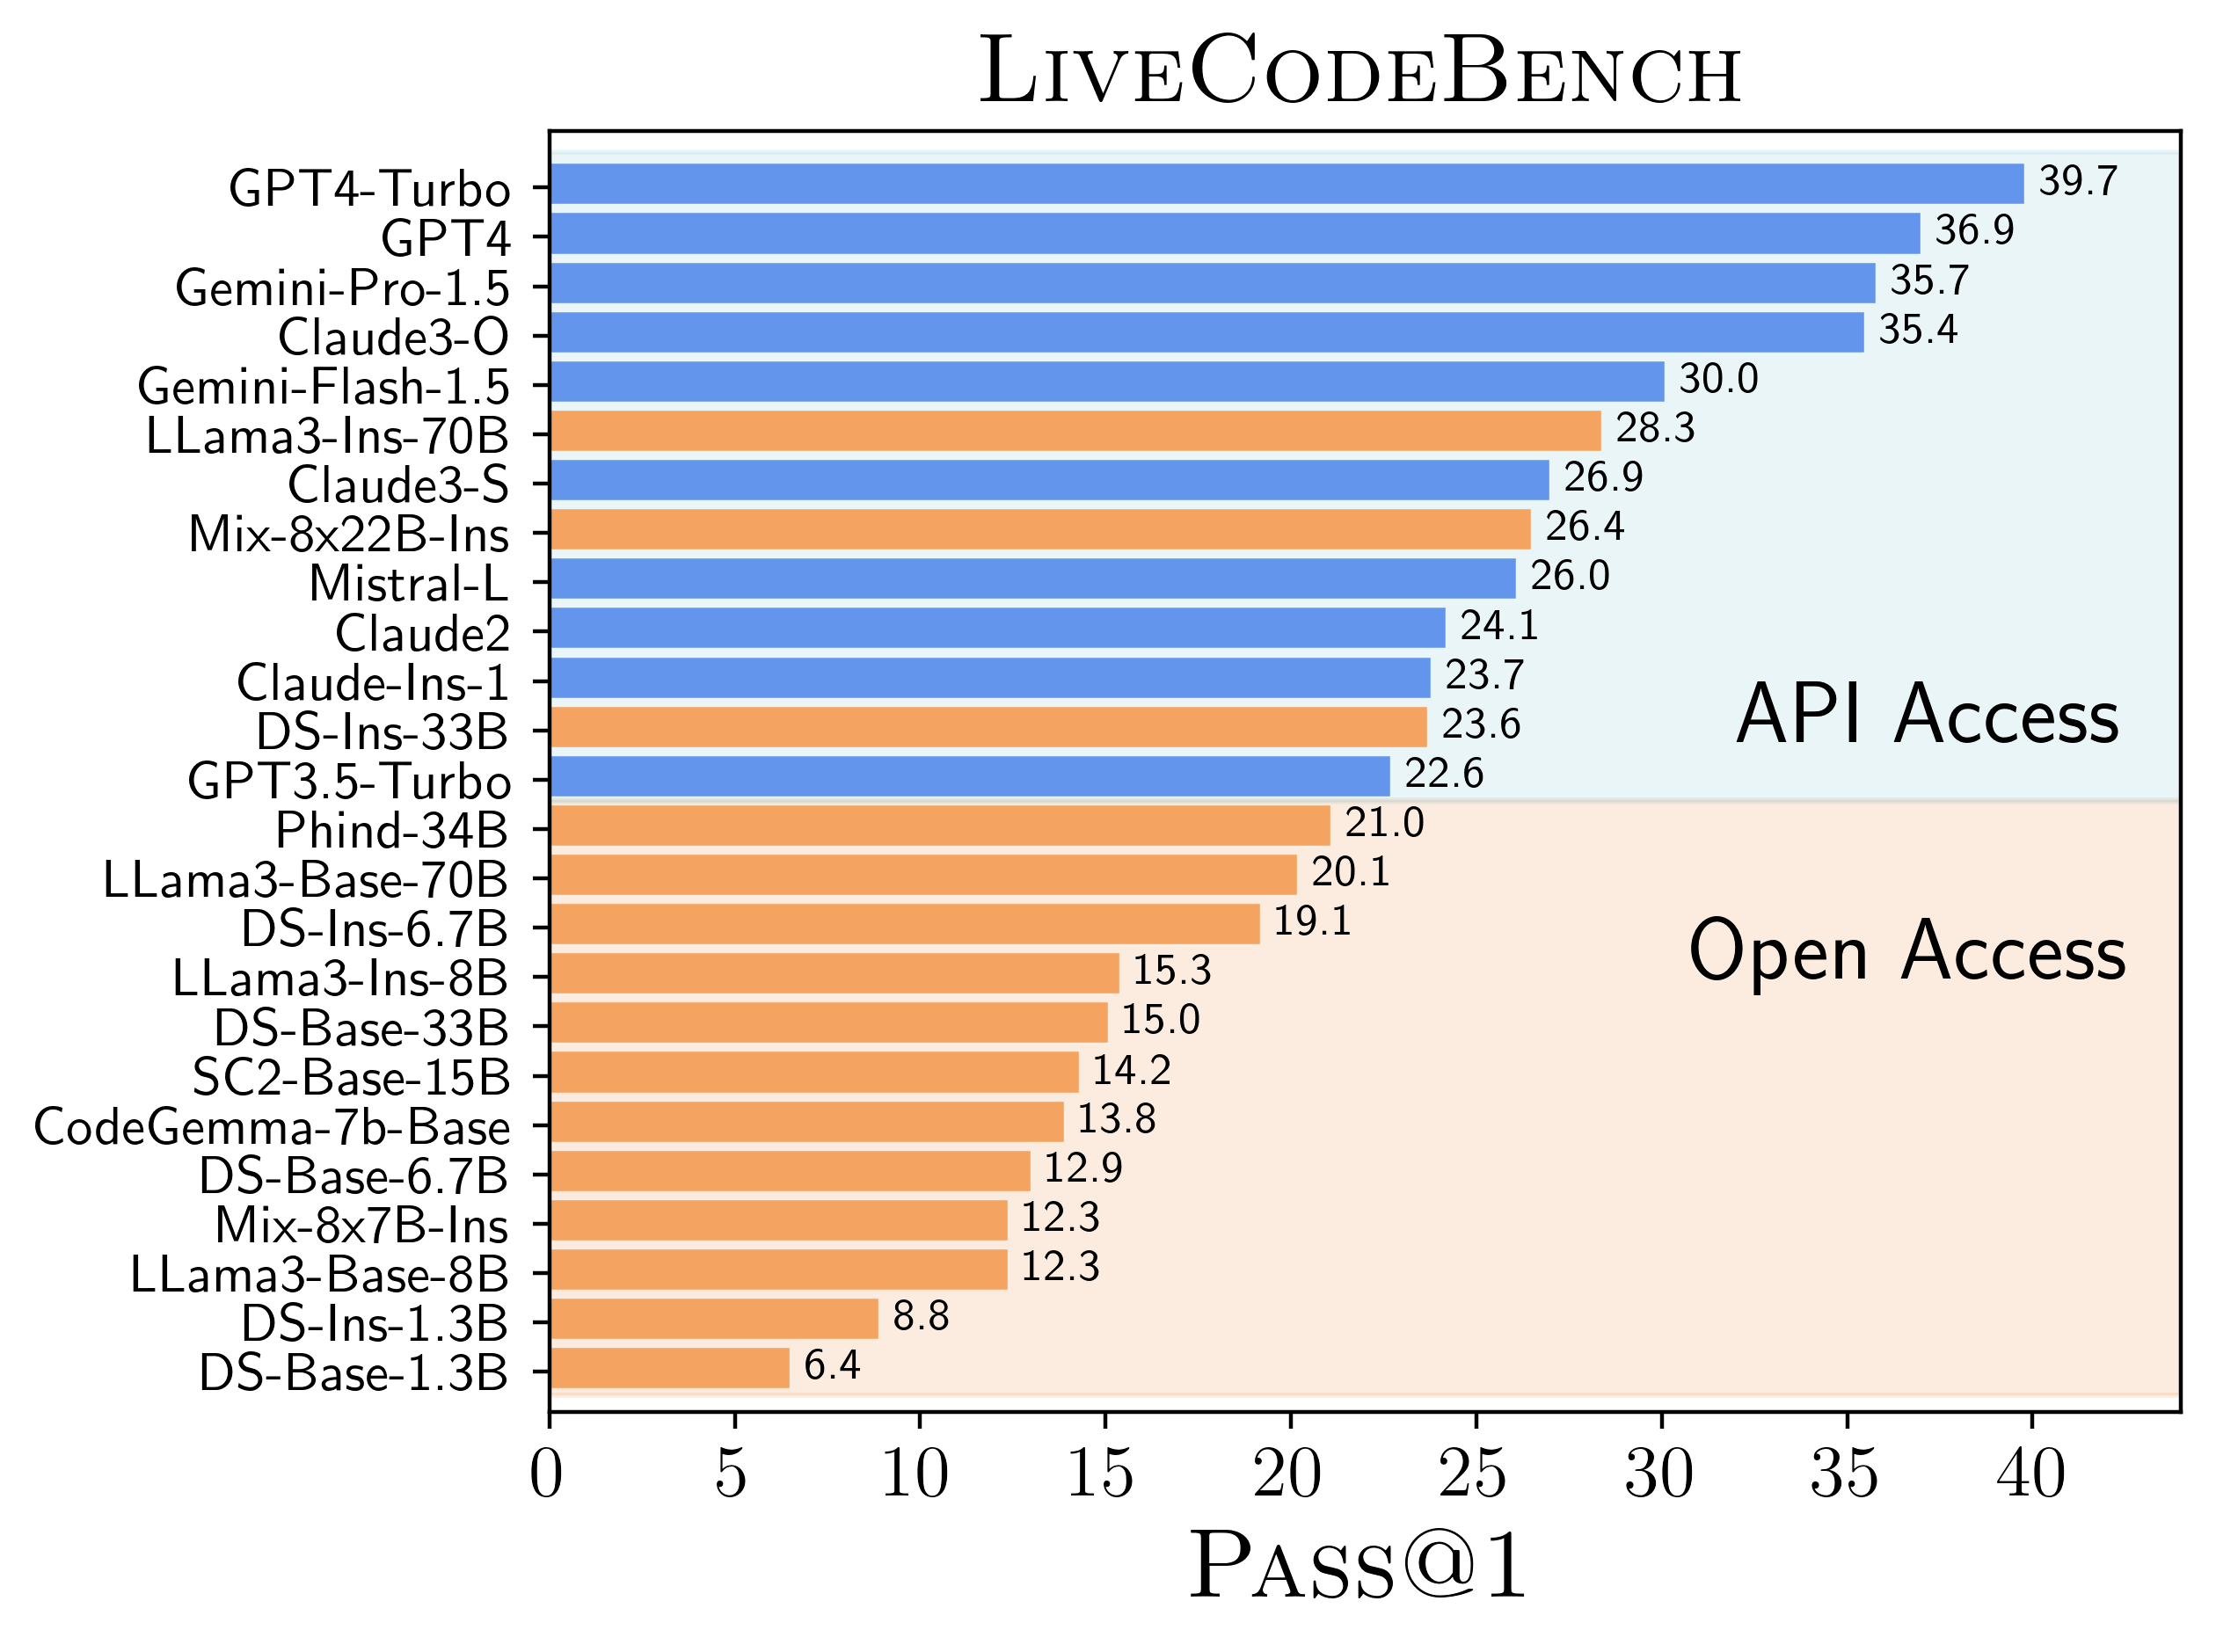
\includegraphics[width=0.52\linewidth]{figures/overview/lc_barchart.png}%
    % 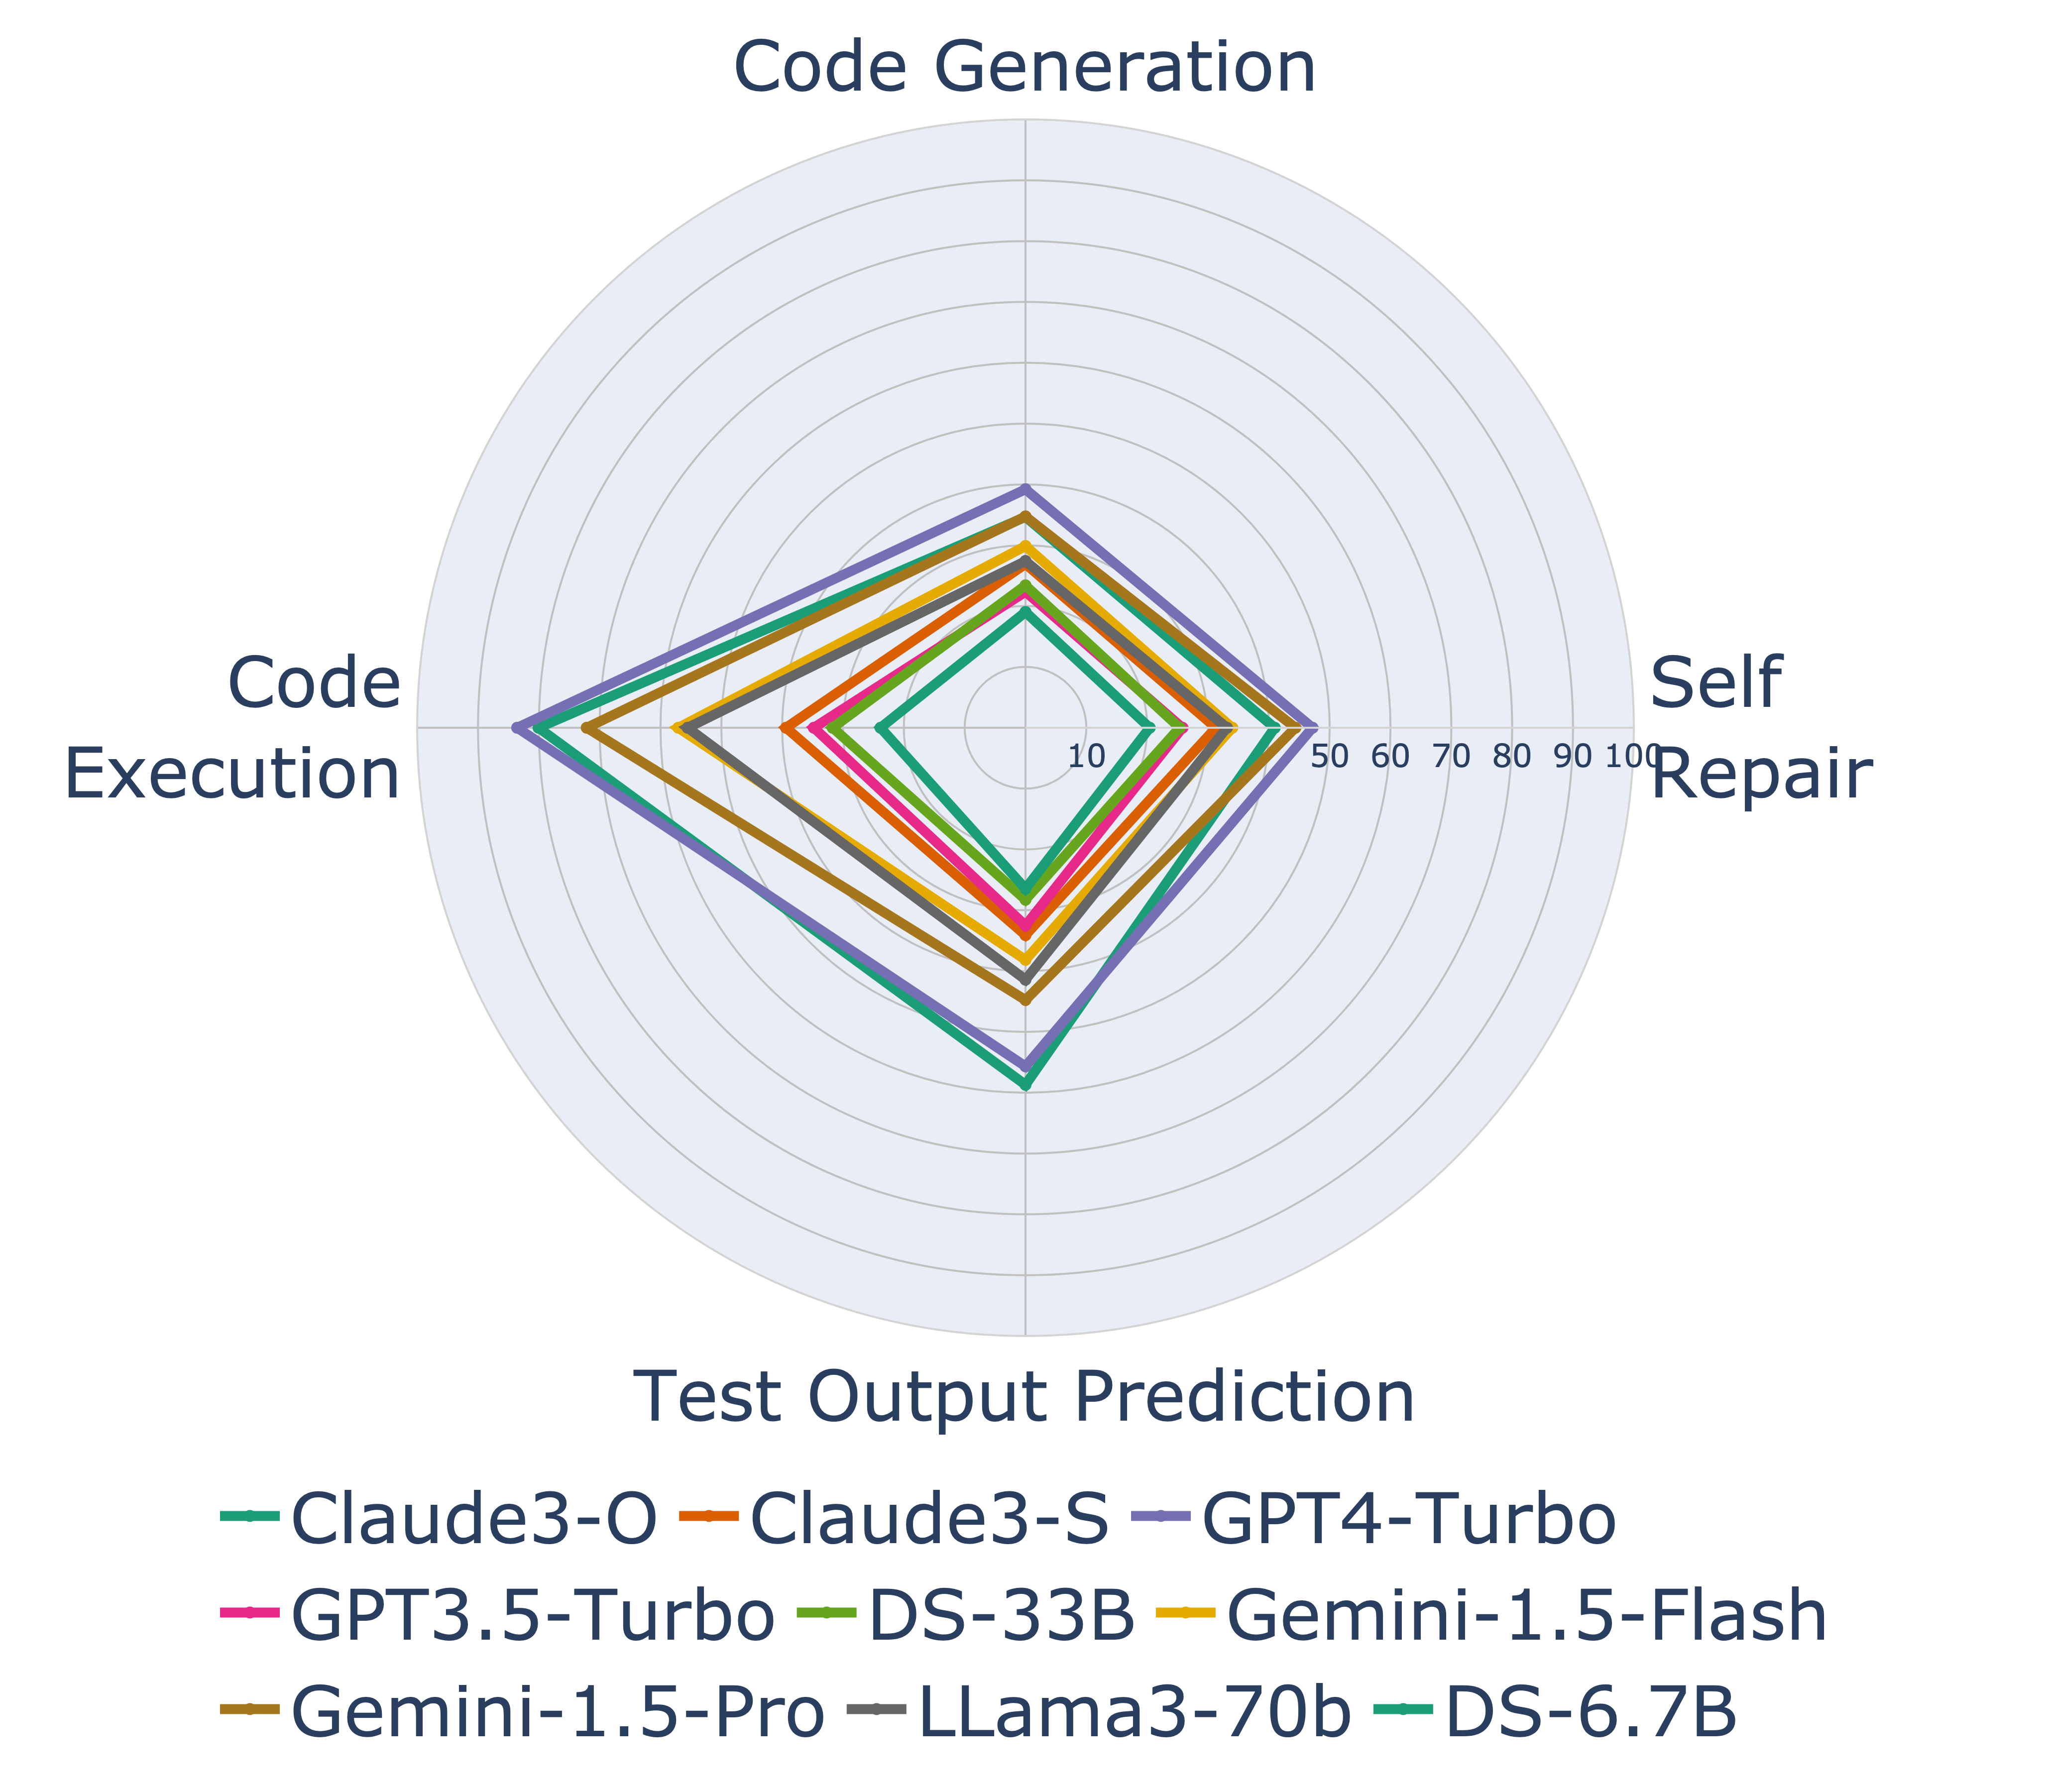
\includegraphics[width=0.5\textwidth]{figures/overview/tasks_radar.png}
    \caption{
        \textbf{Left.} 
        %\ag{maybe make axis 0 to 70 so it doesn't look like test output prediction gets perfect score. also axis labels could be bigger?}
        We propose evaluating \llms{} across 
        scenarios capturing various coding-related capabilities.
        Specifically, we host four different scenarios, namely code generation, 
        self-repair, code execution, and test output prediction.
        The figure depicts various model performances across the four scenarios available in \livecodebench{} in a radial plot -- 
        highlighting how relative differences across models change across the scenarios.
        \textbf{Right.}
        Comparison of open access and (closed) API access models on \livecodebench{}-Easy 
        code generation scenario. We find that closed-access models consistently 
        outperform the open models with only strong instruction-tuned variants of $>30$\textsc{B}
        models (specifically \llamaB{70}, \mixtral and  \deepseekcodeB{33} models) crossing the performance gap.
        }
    \label{fig:all_tasks_radial}
\end{figure}

Motivated by these shortcomings, we introduce \livecodebench{}, built on the following principles:

\begin{enumerate}
\itemsep-0.05em 
    \item \textbf{Live updates to prevent contamination.} 
    \llms{} are trained on massive inscrutable corpora and current benchmarks 
    suffer from the risk of data contamination as they could be included in those training datasets.
While previous works have attempted decontamination using both exact and fuzzy matches~\citep{li2023starcoder, li2023textbooks}, it can be a non-trivial task ~\citep{gemini15,yang2023rethinking}.
        Existing competition programming benchmarks (like \apps{} and \codescope{}) are already contaminated and may fail to provide reliable evaluation of code \llm{} capabilities.
    In \livecodebench{}, to prevent the risk of problem contamination, we evaluate models on \textit{new} problems tagged with a \textit{release date}. 
    Next, for newer models, we only consider problems released after the model's cutoff date to ensure that the model has not been trained on it as demonstrated in Figure~\ref{fig:contamination_main} left.
    %In Figure~\ref{fig:contamination_main} (left), we find that the performance of the \deepseekcodeB{33} and \gptfouro{} starkly  drops on more recent problems released after their cutoff dates and we leverage them for fair evaluations.
    % August $2023$.  
    % Similarly, \gptfouro{} observes a drop in performance on \leetcode{} problems released since November 2023, its specified cutoff date.
    %This indicates that these models are likely trained on the older \leetcode{} problems and time-segmented evaluations allow fair comparisions.
    
    \item \textbf{Holistic Evaluation.} 
    Current code evaluations primarily focus on natural language to code generation.
    However, programming is a multi-faceted task that requires capabilities beyond those measured by code generation. 
    These broader capabilities are even more relevant for constructing programming agents that can interact with the execution environment.
    Therefore, we evaluate the execution-feedback-based multi-turn coding using the self-repair scenario \citep{olausson2023demystifying}, assess code comprehension capabilities using the code execution scenario \citep{gu2024cruxeval}, and introduce the test output prediction scenario to evaluate the models' test generation capabilities.

    \item \textbf{High-quality problems and tests.}
    High-quality problems and tests are crucial for reliable evaluation of \llms{}.
    However, existing benchmarks suffer from multiple deficiencies.
    First, existing competitive programming benchmarks (\apps{}, \contests{}, \xcode{}, \codescope{}) contain problems not amenable to input-output-based auto-grading.
    For example, \contests{} \citep{li2022competition} (page 39, second-to-last paragraph) reports that about twenty-five percent of the problems in the benchmark accept multiple correct outputs for a single input. 
    This \emph{incorrectly penalizes correct solutions}, adding noise to a considerable fraction of the benchmark.
    Next, prior benchmarks like \humaneval{} and \apps{} contain insufficient tests, further exacerbating noise in evaluations ( \citet{liu2023evaluating} reports $8\%$ drop in model performance).
    In \livecodebench{}, we source high-quality problems from reputable platforms and implement heuristics to detect and remove problems not amenable to input-output-based auto-grading.
    Finally, for every problem, we provide a substantial number of tests (over $18$ on average) for reliable and efficient evaluations. In contrast to prior works, we also include several large tests designed for stress-testing solutions ensuring weak or worse complexity solutions do not pass test harnesses.
        
    \item \textbf{Difficulty Guided Problem Curation.} 
    Competitive programming is a challenging domain even for strong \llms{}.
    As a result, these problems can be unsuitable for meaningfully comparing today's open \llms{}, because the variance in performance is low, often relying on less than 1\% performance differences (within the margin of error).
    Therefore, we use problem difficulty ratings (sourced from the competition websites) to curate our problems, avoiding those that are too difficult for current models.
    In particular, we avoid collecting \codeforces{} problems used by prior works (\contests{}, \codescope{}, \xcode{}) since we find they do not sufficiently distinguish models due to model performances (\passmetric{1}) tending to zero.    
    Indeed, \lcb{} easy and medium problems can separate $7$B models that are indistinguishable on the hard subset (see \deepseekcode{7} vs \sctwoinsB{7}).
    
\end{enumerate} 


\begin{table}[!t]
\centering
\caption{Comparing \lcb{} with existing coding and competition programming benchmarks.}
\label{tab:benchmark_comparison}
\resizebox{.95\textwidth}{!}{% 
\begin{tabular}{lccccccc}
  \toprule
  Benchmark & \shortstack{\textbf{Contamination}\\\textbf{Prevention}} & \shortstack{\textbf{Problem}\\\textbf{Curation}} & \shortstack{\textbf{Robust Test}\\\textbf{Based Eval.}} & \shortstack{\textbf{Varied}\\\textbf{Difficulties}} & \shortstack{\textbf{Not}\\\textbf{Saturated}} & \shortstack{\textbf{Broader Eval.}\\\textbf{Scenarios}} & \shortstack{\textbf{Comp. Analysis}\\\textbf{across Models}}   \\
  \midrule
  \humaneval{} \citep{chen2021evaluating} & \xmark & \cmark & \xmark & \cmark & \xmark &  \xmark &  \cmark\\
  \humanevalplus{} \citep{liu2023your} & \xmark & \cmark & \cmark & \cmark & \xmark & \xmark &  \cmark \\
  \mbpp{} \citep{austin2021program} & \xmark & \cmark & \xmark & \cmark & \xmark & \xmark &  \cmark \\
  %\mbppplus{} & \xmark & \cmark & \xmark & \cmark & \xmark \\
  \midrule
  \apps{} \citep{hendrycks2021measuring} & \xmark & \xmark & \xmark & \cmark  & \cmark & \xmark &  \xmark \\
  \contests{} \citep{li2022competition} & \xmark & \xmark & \cmark & \xmark & \cmark & \xmark &  \xmark \\
  \xcode{} \citep{khan2023xcodeeval} & \xmark & \xmark & - & \xmark & \cmark & \cmark \protect\footnotemark[2] &  \xmark \\
  \codescope{} \citep{yan2023codescope} & \xmark & \xmark & - & \xmark & \cmark & \cmark \protect\footnotemark[2] &  \xmark \\
  \taco{} \citep{li2023taco} & \xmark & \xmark & \xmark & \xmark & \cmark & \xmark &  \xmark \\
  \usacobench{} \citep{shi2024language} & \xmark & \cmark & \cmark & \cmark & \cmark & \xmark &  \xmark \\
  \midrule
  \livecodebench{} (Ours) & \cmark & \cmark & \cmark & \cmark & \cmark & \cmark &  \cmark \\
  \bottomrule
\end{tabular}}
    \vspace{-5pt}
\end{table}

\stepcounter{footnote}
\footnotetext{\livecodebench{} considers different evaluation scenarios compared to \xcode{} and \codescope{} focusing on settings where reliable evaluation is possible.}
\vspace{-3pt}
\noindent With these principles in mind, we build \livecodebench{}, a continuously updated benchmark that avoids data contamination.
Particularly, we collect $612$ problems from contests occurring between May $2023$ and Aug $2024$ and use them to construct the different scenarios. 
\newline
\newline
\noindent \textbf{Empirical Findings.} 
We have evaluated over $50$ ($18$ base models and $34$ instruction-tuned) models across different \livecodebench{} scenarios.
Based on this study and following analysis, we present novel empirical findings which have not been revealed in prior benchmarks.
% is revealed be revealed and learned in \livecodebench{} but not in prior benchmarks.
\vspace{-3pt}
\begin{enumerate}
\itemsep-0.05em 
    \item \textbf{Contamination.} 
    We observe a stark drop in the performance of \deepseek{}, \gptfouro{}, \codestral{} and \claudethrees{}  on \leetcode{} problems released after Aug $2023$, Oct $2023$, Jan $2024$, and April $2024$ (Figure~\ref{fig:contamination_main} left). These results highlight likely contamination in older problems and time-segmented evaluations 
    prove effective for performing fair comparisons across varied set of models from both open and closed domains.
    %\nj{gpt4o codestral contamination}
    
    \item \textbf{Holistic Evaluation.} 
    Our evaluations reveal that model performances are correlated across tasks, but the relative differences do vary. 
    For example, in Figure~\ref{fig:contamination_main} right, the gap between open and closed models further increases on tasks like self-repair or test output prediction. 
    Similarly, \claudeopus{} surpasses \gptfour{} on the test output prediction scenario. % This highlights the importance of a holistic evaluation.
    %\nj{update}
    %\ag{i wonder if a table showing task and model rank would show this nicely? and then could also do pairwise correlations between tasks, which would also be interesting to see.}
    
    \item \textbf{\humaneval{} Overfitting.} 
    Upon comparing \livecodebench{} with \humaneval{}, we find that models cluster into two groups, ones that perform well on both benchmarks, and others that perform well on \humaneval{} but not on \livecodebench{} (see Figure~\ref{fig:he_vs_lcb}).
    The latter group primarily comprises fine-tuned open-access models while the former comprises base and closed models.
    This indicates some level of overfitting to \humaneval{}. %\nj{update}

    
    \item \textbf{Model Comparisons} (Figure \ref{fig:results_plots}). We provide model comparisons across different groups like base, instruct, open, and closed models and across groups like open vs closed models.
\end{enumerate}

\vspace{-3pt}
\noindent \textbf{Concurrent Work.} 
~\citep{huang2023competition} also evaluate \llms{} in a time-segmented manner. 
However, they only focus on \codeforces{} problems, while we combine problems across platforms 
and additionally propose a holistic evaluation across multiple code-related scenarios. 
%~\citep{li2023taco} provides a large competition programming dataset but do not study contamination or tasks beyond generation.
~\cite{liu2024codemind} evaluate the code comprehension capabilities of \llms{} using execution. \citep{singhal2024nofuneval} also evaluates \llms{} on more tasks but focus on \textit{non-functional-correctness aspects} of programming. 
~\citet{shi2024language} evaluate \llms{} on USACO problems while we focus on simple competition scenarios.
%beyond code generation, but they consider tasks that take into account the .
%\citep{deepseek-coder} also evaluate \deepseek{} on \leetcode{} problems and mention the possibility of problem contamination.
%\nj{find?}
% in \deepseek{}.

% \begin{table}[t]
% \caption{\small xxx}
% \label{tab:related}
% \begin{center}
% {\scriptsize
% \begin{tabular}{lcccc}
%   \toprule
%   Problem/Method & Bilevel & Multi-objective & Min-max & Single-loop & $\mathcal{X}\subset \R^{d_x}$ \\
%   \midrule
%   Distributionally Robust Learning & $\dagger$ & \xmark & \cmark & - & - \\
%   Adversarially Robust Learning & $\dagger$ & \xmark & \cmark & - & $\triangle$ \\
%   \bottomrule
% \end{tabular}
% }
% \end{center}
% \end{table}
